\documentclass[12pt]{article}
\usepackage[margin=0.8in]{geometry}
\usepackage{amsmath}
\usepackage{hyperref}
\usepackage{graphicx}
\usepackage{float}
\usepackage{caption}
\usepackage{subcaption}
\usepackage{listings}

\title{Numerical analysis: Assignment 10}
\author{Niccolo Zuppichini}
\begin{document}

\maketitle
\section*{Exercise 1}

The code has been implemented in \textit{exercise1.py}. The output of my code is reported in Lst. \ref{lst:output} and in Fig. \ref{fig:output} : \\

\begin{lstlisting}[caption=Code output, label=lst:output]
It took 110 iterations to get an error of the residual (abs norm) 
of 2.7286568582057953
The least squares solution is point P: [0.85714272 0.71428582]; 
with the weights: [1.0581167  5.617022   0.94311583 1.8340678 ] 
\end{lstlisting}
%
\begin{figure}[h]\texttt{
\centering
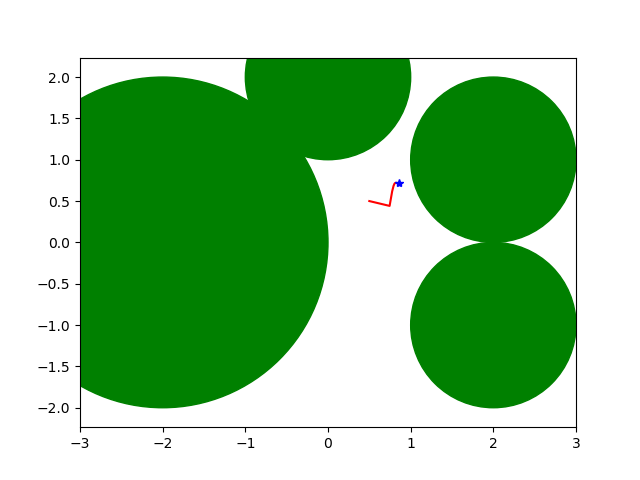
\includegraphics[width = 0.7 \linewidth]{plot.png}
\caption{Iterations up to convergence from initial guess [0.5, 0.5]}
\label{fig:output}}
\end{figure}

 Observe Image \ref{fig:output} we can see a "90 degree shape" of the path. Because we are using only first order information it's normal to have this kind of path. Figure \ref{fig:output2} shows it more closely. If we used second order information we wouldn't see this "90 degree shape" but rather a more "smooth path" to the least square solution (the black path shows in Figure \ref{fig:output2}). \\

\begin{figure}[h]\texttt{
\centering
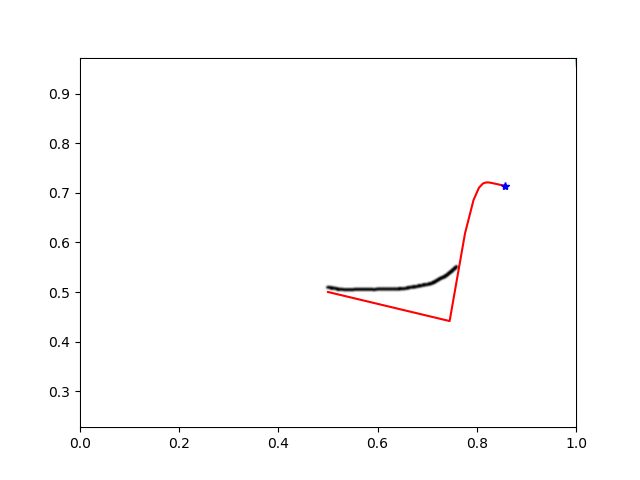
\includegraphics[width = 0.7 \linewidth]{plot2.png}
\caption{Close-up to the iterations and what the path (more or less) should look like using second order information}
\label{fig:output2}}
\end{figure}


\end{document}